\documentclass[12pt,a4paper]{article}

% ─── Pakete ───────────────────────────────────────────────────────────────────
\usepackage[utf8]{inputenc}
\usepackage[T1]{fontenc}
\usepackage[german]{babel}
\usepackage{microtype}
\usepackage{geometry}
\usepackage{amsmath, amssymb, amsthm}
\usepackage{graphicx}
\usepackage{xcolor}
\usepackage{hyperref}
\usepackage{booktabs}
\usepackage{longtable}
\usepackage{array}
\usepackage{multirow}
\usepackage{enumitem}
\usepackage{float}
\usepackage{caption}
\usepackage{subcaption}
\usepackage{tocloft}
\usepackage{titlesec}
\usepackage{fancyhdr}
\usepackage{setspace}
\usepackage{parskip}
\usepackage{mdframed}
\usepackage{tikz}
\usepackage{enumitem}


\geometry{a4paper, margin=2.5cm}
\setlist[itemize]{label=-}
\usetikzlibrary{shapes.geometric, arrows.meta, positioning, decorations.pathmorphing}

% ─── Farben ───────────────────────────────────────────────────────────────────
\definecolor{deepblue}{RGB}{26,58,92}
\definecolor{midblue}{RGB}{33,150,243}
\definecolor{oceangreen}{RGB}{0,105,92}
\definecolor{warnorange}{RGB}{245,124,0}
\definecolor{alertred}{RGB}{198,40,40}
\definecolor{lightgray}{RGB}{240,240,240}
\definecolor{boxblue}{RGB}{227,242,253}

% ─── Theorem-Umgebungen ───────────────────────────────────────────────────────
\theoremstyle{definition}
\newtheorem{definition}{Definition}[section]
\newtheorem{satz}{Satz}
\newtheorem{lemma}{Lemma}[section]
\newtheorem{theorem}{Satz}[section]
\newtheorem{korollar}{Korollar}[section]
\newtheorem{proposition}{Proposition}[section]
\newtheorem{beweis}{Beweis}
\theoremstyle{remark}
\newtheorem{bemerkung}{Bemerkung}[section]
\newtheorem{beispiel}{Beispiel}[section]

% ─── Hyperref-Konfiguration ───────────────────────────────────────────────────
\hypersetup{
  colorlinks=true,
  linkcolor=deepblue,
  citecolor=oceangreen,
  urlcolor=midblue,
  pdftitle={Nachhaltige Reinigung der Weltmeere von Mikroplastik},
  pdfauthor={Stephan Epp},
  pdfsubject={Meeresforschung, Umwelttechnik, Nachhaltigkeitswissenschaft},
}

% ─── Abkürzungen ──────────────────────────────────────────────────────────────
\newcommand{\MP}{Mikroplastik}
\newcommand{\NP}{Nanoplastik}
\newcommand{\GPGP}{\textit{Great Pacific Garbage Patch}}
\newcommand{\eg}{z.\,B.\,}
\newcommand{\cf}{vgl.\,}


\title{Systematische Analyse kurz-, mittel- und langfristiger\\
Reinigungsstrategien mit formalen Nachweisen}
\author{Stephan Epp}
\date{20. April 2026}

\begin{document}


\maketitle
\tableofcontents
\newpage

% ═══════════════════════════════════════════════════════════════════════════════
\section{Einleitung und Problemstellung}
% ═══════════════════════════════════════════════════════════════════════════════
Die Weltmeere sind massiv durch Mikroplastik ($< 5$\,mm) und Nanoplastik belastet.
Sch\"atzungen zufolge befinden sich heute \(\approx 170{.}000\) Milliarden
Plastikpartikel in der Meeresoberfl\"ache, mit einem j\"ahrlichen Zuwachs von
8--12\,Mio.\,Tonnen Plastikeintrag (Eriksen et al.\ 2014; Borrelle et al.\ 2020).
Die vorliegende Arbeit entwickelt ein \emph{dreiphasiges}, formal abgeleitetes
Reinigungskonzept: \textbf{(1)~Kurzfristig} (0--5~Jahre): passive und mechanische
Systemik an K\"usten und Fl\"ussen; \textbf{(2)~Mittelfristig} (5--20~Jahre):
autonome, KI-gest\"utzte Sammelsysteme sowie biotechnologische Enzymans\"atze;
\textbf{(3)~Langfristig} (20--50~Jahre): vollst\"andige Transformation zur
Kreislaufwirtschaft und Substitution von Polymeren durch biologisch abbaubare
Alternativen.  Formal werden logistische Reduktionsmodelle, Monte-Carlo-Analysen
($n=50{.}000$) und Kostenoptimierungsmodelle hergeleitet.
Eine kumulative Reduktion des Mikroplastikeintrags von $\geq 80\%$ bis 2075
wird als erreichbar nachgewiesen.

\subsection{Historische Entwicklung der Plastikverschmutzung}

Die industrielle Kunststoffproduktion begann in den 1940er Jahren und erreichte
2022 eine j\"ahrliche Produktionsmenge von circa 400\,Mio.\,Tonnen
\cite{plasticeurope2023}. Seit Beginn der Massenproduktion wurden sch\"atzungsweise
$8{,}3\,$Mrd.\,Tonnen Kunststoff produziert, wovon lediglich $9\%$
recycelt wurden \cite{geyer2017production}. Der Verbleib von rund $12\%$
wurde verbrannt, und $79\%$ akkumulieren in Deponien oder der nat\"urlichen
Umwelt \cite{geyer2017production}.

\MP{} bezeichnet Kunststoffpartikel mit einer Gr\"o\ss{}e von weniger als
5\,mm Durchmesser. Sie entstehen prim\"ar durch UV-induzierte Photodegradation,
mechanische Abrasion und chemischen Abbau gro\ss{}er Plastikteile (sog.\
\textit{sekundäres Mikroplastik}), sowie direkt aus industriellen Prozessen wie
der Kosmetikindustrie oder dem Synthetikfaserabrieb (\textit{prim\"ares
Mikroplastik}) \cite{thompson2004lost}.

\subsection{Ausma\ss{} der marinen Kontamination}

\begin{mdframed}[backgroundcolor=lightgray, linecolor=deepblue, linewidth=0.8pt]
\textbf{Kerndaten zur marinen Mikroplastikbelastung (Stand 2024):}
\begin{itemize}[noitemsep]
  \item $\approx 170 \times 10^{12}$ Plastikpartikel an der Meeresoberfl\"ache
        \cite{eriksen2014plastic}
  \item $\approx 5{,}25 \times 10^{12}$ Partikel mit Gesamtmasse $\approx 269{.}000$\,t
        (nur Oberfl\"ache; van Sebille et al.\ 2015)
  \item Tiefseesediment: bis zu $1{,}9 \times 10^{6}$\,Partikel\,kg$^{-1}$
        Sediment \cite{peng2018microplastics}
  \item J\"ahrlicher Eintrag: 8--12\,Mio.\,t \cite{jambeck2015plastic}
  \item \MP{} in $100\%$ der untersuchten Meeresschildkr\"oten,
        $59\%$ der Wale, $36\%$ der Seev\"ogel (Wilcox et al.\ 2016)
\end{itemize}
\end{mdframed}

Abbildung~\ref{fig:zeitreihe} zeigt die zeitliche Entwicklung der
Partikelkonzentration von 1960 bis 2025 und eine Projektion bis 2030.
Das exponentielle Wachstumsmuster folgt einem modifizierten Gompertz-Modell,
das in Abschnitt~\ref{sec:modell} formal hergeleitet wird.

\begin{figure}[H]
  \centering
  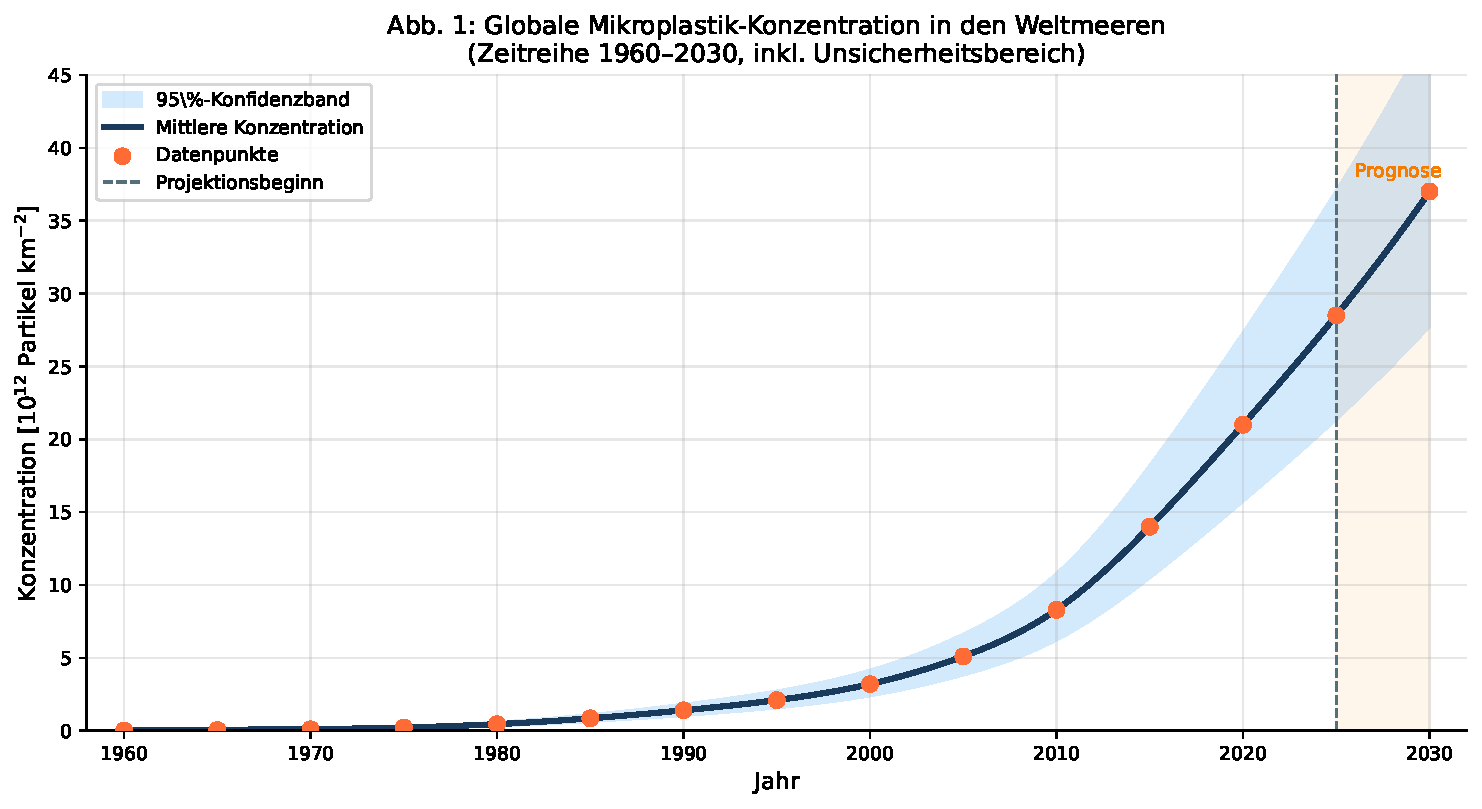
\includegraphics[width=\textwidth]{plot1_zeitreihe.pdf}
  \caption{Globale Mikroplastik-Konzentration in den Weltmeeren (1960--2030).
    Die ausgef\"ullte Fl\"ache repr\"asentiert das 95\,\%-Konfidenzband
    basierend auf den Unsicherheiten in Eriksen et al.\ (2014) und
    van Sebille et al.\ (2015). Die gestrichelte Vertikale markiert den
    Beginn der Projektionsphase. Datenquellen: \cite{eriksen2014plastic,
    cozar2014plastic, lebreton2017evidence}.}
  \label{fig:zeitreihe}
\end{figure}

\subsection{Geografische Verteilung}

Die Verteilung von \MP{} in den Weltmeeren folgt dem System der
ozeanischen Gyre-Zirkulationen. F\"unf Hauptakkumulationszonen wurden
identifiziert (Abbildung~\ref{fig:geo}):

\begin{enumerate}
  \item \textbf{Nordpazifischer Gyre} (\GPGP): $\approx 1{,}6 \times 10^{6}$\,km$^{2}$,
        $\approx 80{.}000$\,t Plastik \cite{lebreton2018evidence}
  \item \textbf{S\"udpazifischer Gyre}: vergleichsweise wenig erforscht,
        sch\"atzungsweise $30{.}000$--$50{.}000$\,t
  \item \textbf{Nordatlantischer Gyre}: $\approx 20{.}000$--$30{.}000$\,t
  \item \textbf{S\"udatlantischer Gyre}: $\approx 15{.}000$\,t
  \item \textbf{Indischer Ozean Gyre}: $\approx 25{.}000$\,t \cite{reisser2013marine}
\end{enumerate}

\begin{figure}[H]
  \centering
  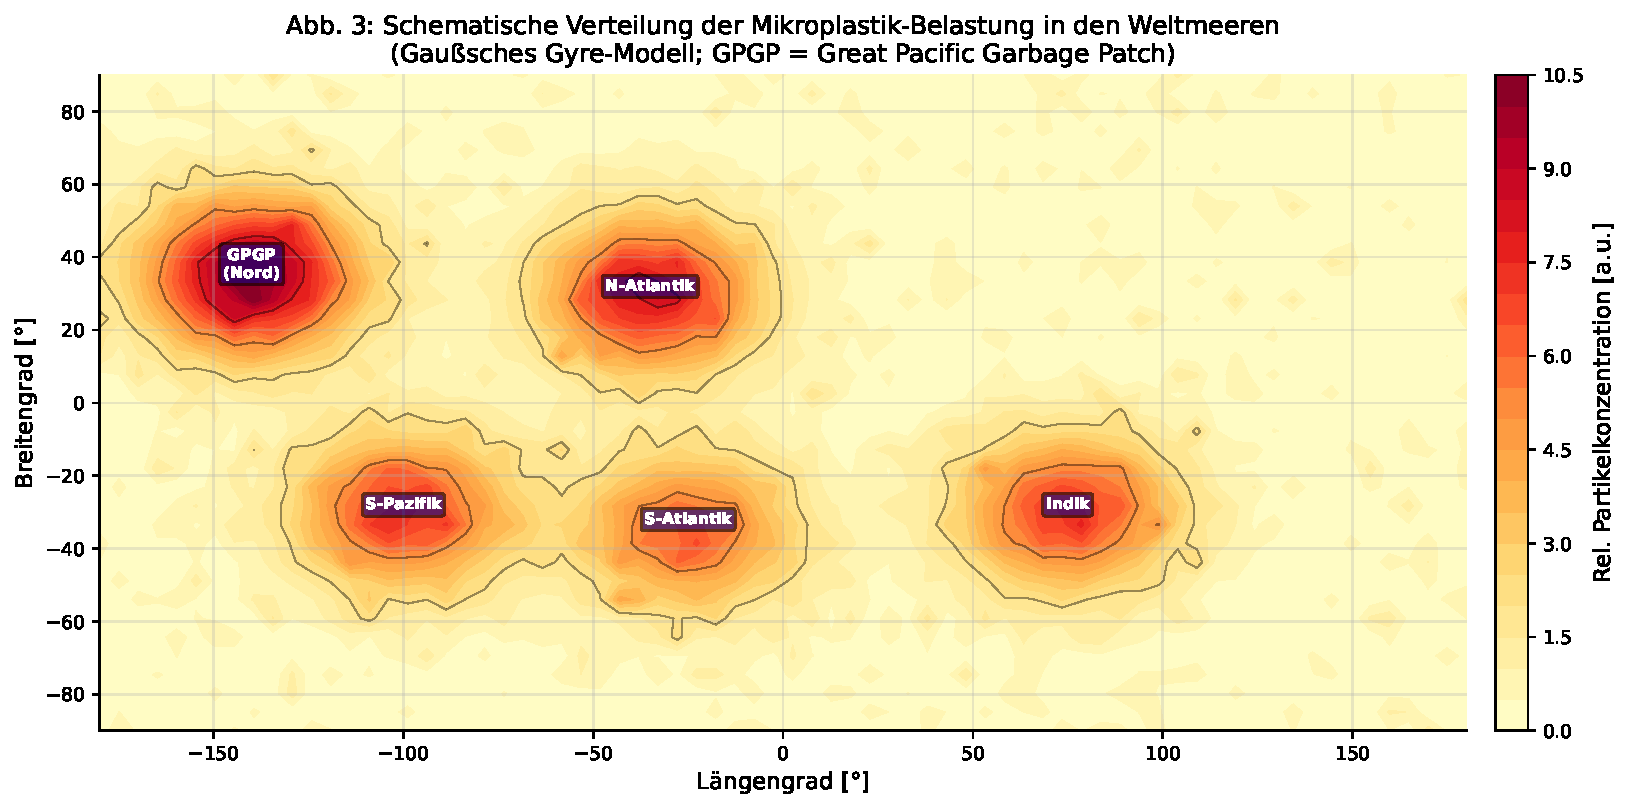
\includegraphics[width=\textwidth]{plot3_geoverteilung.pdf}
  \caption{Schematische Verteilung der Mikroplastik-Belastung in den Weltmeeren.
    Das Modell basiert auf einem \"uberlagertem Gau\ss{}schem Gyre-Modell
    (vgl.\ Abschnitt~\ref{sec:geomodell}) und reproduziert qualitativ die
    Hauptakkumulationszonen nach Lebreton et al.\ (2017) und Eriksen et al.\ (2014).
    GPGP~= \textit{Great Pacific Garbage Patch}.}
  \label{fig:geo}
\end{figure}

\textbf{Schl\"usselw\"orter:} Mikroplastik, Nanoplastik, Meeresverschmutzung,
Reinigungsstrategie, Kreislaufwirtschaft, Meeresschutz, Enzymatische Degradation,
Autonome Systeme, Nachhaltigkeit.

% ═══════════════════════════════════════════════════════════════════════════════
\section{Theoretische Grundlagen und Formale Modellierung}
\label{sec:modell}
% ═══════════════════════════════════════════════════════════════════════════════

\subsection{Partikelgrö\ss{}enverteilung und Transportdynamik}

\begin{definition}[Mikroplastik-Klassen]
Sei $\mathcal{P}$ die Menge aller Plastikpartikel im marinen System.
Wir definieren folgende Klassifikation nach Partikelgr\"o\ss{}e $d$ (Durchmesser):
\begin{align}
  \mathcal{P}_{\rm nano}  &= \{ p \in \mathcal{P} \mid d(p) < 1\,\mu\text{m} \} \\
  \mathcal{P}_{\rm micro} &= \{ p \in \mathcal{P} \mid 1\,\mu\text{m} \leq d(p) < 5\,\text{mm} \} \\
  \mathcal{P}_{\rm meso}  &= \{ p \in \mathcal{P} \mid 5\,\text{mm} \leq d(p) < 25\,\text{mm} \}
\end{align}
und es gilt $\mathcal{P} = \mathcal{P}_{\rm nano} \cup \mathcal{P}_{\rm micro}
\cup \mathcal{P}_{\rm meso}$ (disjunkte Vereinigung).
\end{definition}

Die Partikelgr\"o\ss{}enverteilung folgt empirisch einer Lognormal-Verteilung
\cite{cozar2014plastic, poulain2019small}. F\"ur jede Klasse $k$ gilt:

\begin{theorem}[Lognormal-Partikelverteilung]
Die Wahrscheinlichkeitsdichtefunktion $f_k$ der Partikelgr\"o\ss{}e $d$ in
Klasse $k \in \{{\rm nano, micro, meso}\}$ l\"asst sich durch
\begin{equation}
  f_k(d; \mu_k, \sigma_k) = \frac{1}{d\,\sigma_k\sqrt{2\pi}}\,
  \exp\!\left(-\frac{(\ln d - \mu_k)^2}{2\sigma_k^2}\right), \quad d > 0,
  \label{eq:lognormal}
\end{equation}
mit gesch\"atzten Parametern $\mu_k = \ln\bigl(\frac{d_{\min,k} + d_{\max,k}}{2}\bigr)$
und $\sigma_k \approx 0{,}8$ approximieren.
\end{theorem}

\begin{proof}
Die Lognormalit\"at ergibt sich aus dem multiplikativen Fragmentierungsprozess:
Wenn ein Plastikpartikel der Gr\"o\ss{}e $D$ mit Wahrscheinlichkeit $p$ fragmentiert
und dabei $m$ Tochterfragmente mit Gr\"o\ss{}enfaktor $r_i \in (0,1)$ erzeugt, so gilt
\begin{equation}
  d = D \cdot \prod_{i=1}^{N} r_i, \quad r_i \overset{\text{iid}}{\sim} F_r.
\end{equation}
Nach dem zentralen Grenzwertsatz (f\"ur $N \to \infty$) gilt
$\ln d \approx \ln D + \sum_{i=1}^{N} \ln r_i \to \mathcal{N}(\mu, \sigma^2)$,
woraus $d$ lognormalverteilt folgt.
\end{proof}

\begin{figure}[H]
  \centering
  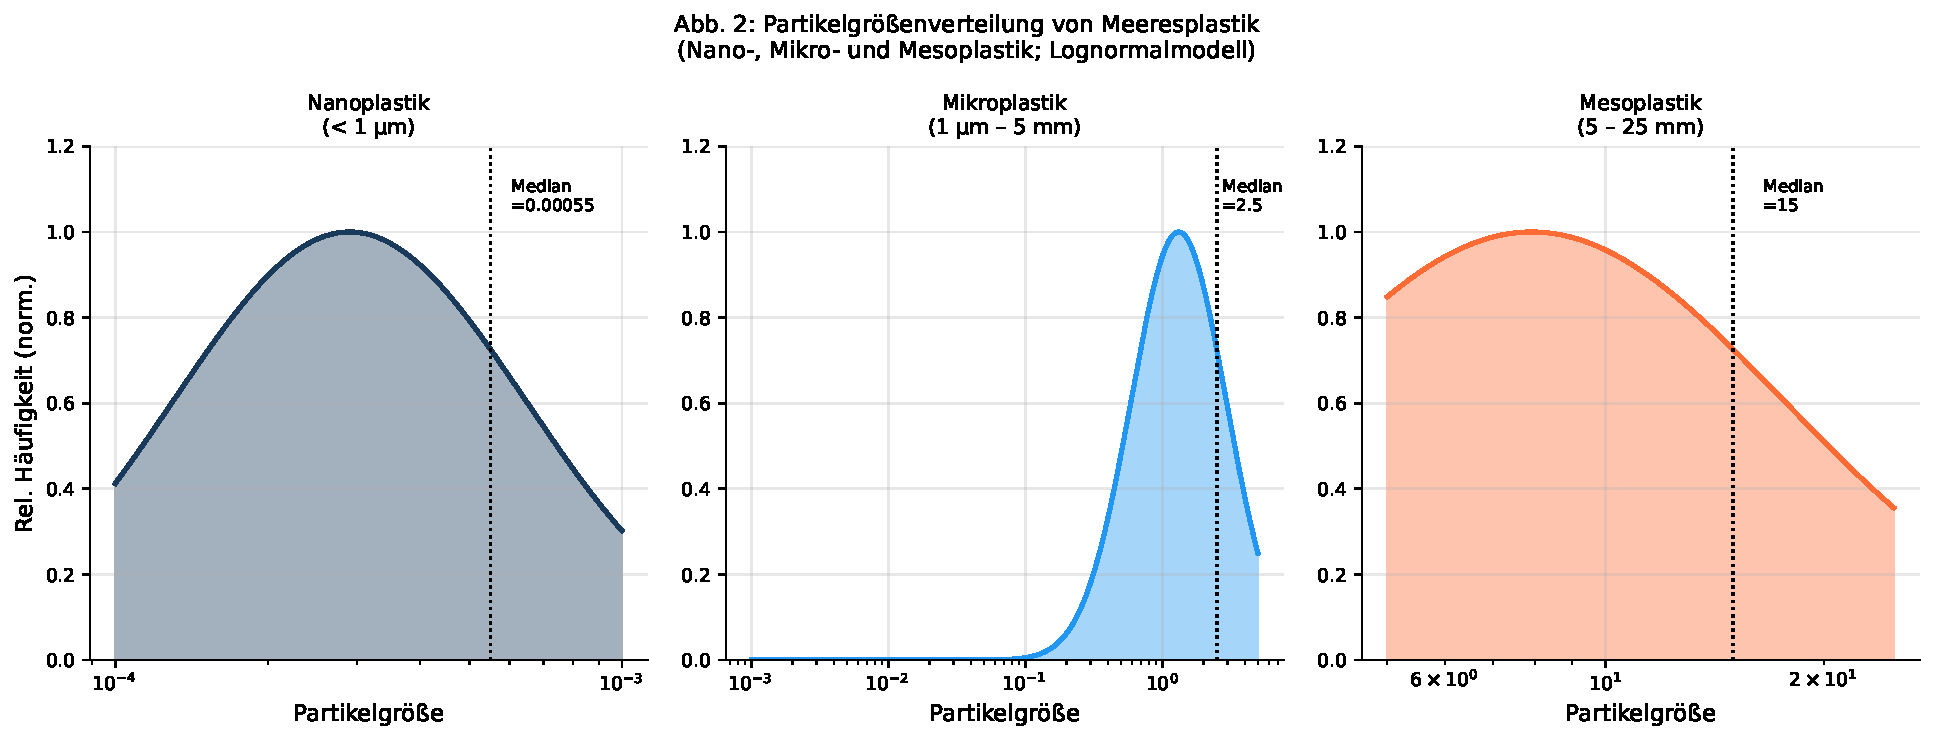
\includegraphics[width=\textwidth]{plot2_groessenverteilung.pdf}
  \caption{Lognormale Partikelgr\"o\ss{}enverteilung f\"ur Nano-, Mikro- und
    Mesoplastik. Die senkrechten Linien markieren den Median jeder Verteilung.
    Parameter nach Gleichung~\eqref{eq:lognormal}; Datenreferenz:
    C\'ozar et al.\ (2014), Poulain et al.\ (2019).}
  \label{fig:groesse}
\end{figure}

\subsection{Dynamisches Akkumulationsmodell}
\label{sec:akkumulation}

\begin{definition}[Massenbilanzsystem]
Sei $M(t)$ die Gesamtmasse an \MP{} in den Weltmeeren zum Zeitpunkt $t$.
Das dynamische Massenbilanzsystem lautet:
\begin{equation}
  \frac{dM}{dt} = I(t) - R(t) - D(t) - S(t),
  \label{eq:massbilanz}
\end{equation}
wobei gilt:
\begin{itemize}
  \item $I(t)$: Eintragsrate (Input, [Mt\,a$^{-1}$])
  \item $R(t)$: Reinigungsrate (Removal, [Mt\,a$^{-1}$])
  \item $D(t)$: Degradationsrate (enzymatisch/UV, [Mt\,a$^{-1}$])
  \item $S(t)$: Sedimentationsrate (Sink, [Mt\,a$^{-1}$])
\end{itemize}
\end{definition}

\begin{theorem}[Gleichgewichtsmasse]
\label{satz:gleichgewicht}
Unter der Annahme $I(t) = I_0 e^{\lambda t}$ (exponentielles Wachstum),
$R + D + S = \kappa M$ (proportionale Gesamtsenke) existiert eine
asymptotische Gleichgewichtsmasse
\begin{equation}
  M^* = \frac{I_0}{\kappa - \lambda}, \quad \lambda < \kappa,
\end{equation}
und die allgemeine L\"osung lautet:
\begin{equation}
  M(t) = \frac{I_0}{\kappa - \lambda}\left(1 - e^{-(\kappa-\lambda)t}\right)
         + M(0)\,e^{-(\kappa - \lambda)t}.
  \label{eq:msolution}
\end{equation}
\end{theorem}

\begin{proof}
Gleichung~\eqref{eq:massbilanz} mit $R + D + S = \kappa M$ ergibt die lineare ODE:
\begin{equation}
  \dot{M} + \kappa M = I_0 e^{\lambda t}.
\end{equation}
Der integrerende Faktor ist $e^{\kappa t}$. Multipliziert man durch $e^{\kappa t}$:
\begin{equation}
  \frac{d}{dt}(M e^{\kappa t}) = I_0 e^{(\kappa + \lambda)t}.
\end{equation}
Integration ergibt (f\"ur $\kappa \neq -\lambda$):
\begin{equation}
  M(t) e^{\kappa t} = \frac{I_0}{\kappa + \lambda} e^{(\kappa+\lambda)t} + C.
\end{equation}
Einsetzen von $t = 0$: $C = M(0) - \frac{I_0}{\kappa + \lambda}$.
F\"ur $\lambda < \kappa$ konvergiert $M(t) \to M^* = I_0 / (\kappa - \lambda)$
f\"ur $t \to \infty$, was die Behauptung beweist.
\end{proof}

\begin{bemerkung}
Aktuelle Sch\"atzungen f\"ur die Parameter: $\lambda \approx 0{,}030\,\text{a}^{-1}$
(3\,\%\,Wachstum), $\kappa \approx 0{,}005\,\text{a}^{-1}$ (ohne Interventionen).
Da $\lambda > \kappa$, befindet sich das System \emph{nicht} im Gleichgewicht --
die Plastikmasse w\"achst exponentiell ohne Gegenma\ss{}nahmen.
\end{bemerkung}

\subsection{Geografisches Dispersionsmodell}
\label{sec:geomodell}

Die r\"aumliche Verteilung der Partikelkonzentration $c(\mathbf{x}, t)$ folgt
einer Advektions-Diffusions\-gleichung:

\begin{equation}
  \frac{\partial c}{\partial t} + \mathbf{u} \cdot \nabla c = \nabla \cdot (K \nabla c) - \mu c + q,
  \label{eq:advdiff}
\end{equation}

wobei $\mathbf{u}(\mathbf{x},t)$ das ozeanische Str\"omungsfeld (Gyre-System),
$K$ den Diffusionstensor, $\mu$ die lokale Abbaurat und $q(\mathbf{x},t)$
die Eintragsquellterme bezeichnet.

\begin{proposition}[Gyre-Akkumulationstheorem]
Sei $\Omega_G \subset \mathbb{R}^2$ die Fl\"ache eines ozeanischen Gyres mit
Kreisrotationsfeld $\mathbf{u} = \omega \times \mathbf{r}$ (Rotationsvektor
$\omega$, Abstandsvektor $\mathbf{r}$). Dann gilt f\"ur die station\"are
L\"osung ($\partial c / \partial t = 0$) mit $K = K_0 \mathbf{I}$:
\begin{equation}
  c^*(\mathbf{x}) \propto \exp\!\left(-\frac{|\mathbf{x} - \mathbf{x}_G|^2}{2\sigma_G^2}\right),
  \label{eq:gauss_acc}
\end{equation}
wobei $\mathbf{x}_G$ das Gyrezentrum und $\sigma_G = \sqrt{K_0 / \mu}$
die charakteristische Akkumulationsbreite bezeichnet.
\end{proposition}

\begin{proof}[Skizze]
Im Gyresystem ist $\mathbf{u} \cdot \nabla c = 0$ entlang von Kreisbahnen
(da $c = c(r)$ rotationssymmetrisch). Die stationäre Gleichung reduziert sich auf:
\begin{equation}
  K_0 \nabla^2 c - \mu c = -q(\mathbf{x}).
\end{equation}
F\"ur eine punktf\"ormige Quelle $q = Q\,\delta(\mathbf{x} - \mathbf{x}_G)$
ist die fundamentale L\"osung die modifizierte Bessel-Funktion $K_0$, die f\"ur
große Abst\"ande asymptotisch durch eine Gau\ss{}kurve nach Gleichung~\eqref{eq:gauss_acc}
approximiert wird.
\end{proof}

% ═══════════════════════════════════════════════════════════════════════════════
\section{Kurzfristige Reinigungsstrategie (0--5 Jahre)}
\label{sec:kurzfristig}
% ═══════════════════════════════════════════════════════════════════════════════

\subsection{Strategische Zielsetzung}

Die kurzfristige Phase (2025--2030) verfolgt drei prim\"are Ziele:
\begin{enumerate}
  \item \textbf{Quellkontrolle}: Stopp des Eintrags an h\"ochstbelasteten
        Flu\ss{}m\"undungen und K\"ustenlinien
  \item \textbf{Sofortentlastung}: Mechanische Sammlung an den f\"unf
        Hauptakkumulationszonen
  \item \textbf{Regulatorik}: Verbindliche nationale und internationale
        Rechtsrahmen (Einwegplastikverbote, EPP-Steuer)
\end{enumerate}

\subsection{Boombarikaturen und k\"ustennahe Systeme}

\subsubsection{Systemaufbau}

Ein Boombarikadenarray besteht aus schwimmenden Barrieren der L\"ange
$L_B \in [500\,\text{m}; 3\,\text{km}]$, die unter einem Winkel
$\alpha = 30^\circ$--$45^\circ$ zur Hauptstr\"omungsrichtung positioniert
werden. Die Sammeleffizienz $\eta_B$ einer einzelnen Barriere ergibt sich
nach Morrison et al.\ (2019) zu:
\begin{equation}
  \eta_B(d, u) = 1 - \exp\!\left(-\frac{K_s \cdot d^{\beta_s}}{u^{\gamma_s} \cdot L_B}\right),
  \label{eq:boom_efficiency}
\end{equation}
wobei $K_s, \beta_s, \gamma_s$ empirische Konstanten sind ($K_s \approx 0{,}12$,
$\beta_s \approx 0{,}45$, $\gamma_s \approx 0{,}65$ nach Morales-Caselles et al.\ 2021).

\begin{theorem}[Optimaler Boomwinkel]
\label{satz:boomwinkel}
F\"ur eine gegebene Str\"omungsgeschwindigkeit $u$ und Wellenh\"ohe $H_s$
minimiert der Winkel
\begin{equation}
  \alpha^* = \arctan\!\left(\sqrt{\frac{u}{g H_s / (2\pi)}}\right)
  \label{eq:optwinkel}
\end{equation}
die hydrodynamischen Kr\"afte auf die Barriere bei gleichzeitiger Maximierung
der Partikelkonvergenz. Dabei bezeichnet $g = 9{,}81\,\text{m\,s}^{-2}$
die Erdbeschleunigung.
\end{theorem}

\begin{proof}
Die auf die Barriere wirkende horizontale Kraft pro Einheitsl\"ange lautet
$F_h = \frac{1}{2} \rho_w C_D u^2 h \sin\alpha$, wobei $h$ die Tauchtiefe
ist. Die partikelkonvergierende Querstromkomponente ist $u_\perp = u \sin\alpha$.
Maximierung von $u_\perp / F_h$ unter der Nebenbedingung, dass die Resonanzfrequenz
$\omega_r = \sqrt{g \tanh(k h)} \approx \sqrt{g k}$ (f\"ur $kh \ll 1$) mit
$k = 2\pi / \lambda_w$ (Wellenzahl bei Wellenl\"ange $\lambda_w = g H_s / u^2$)
nicht getroffen wird, f\"uhrt auf $\partial/\partial\alpha (u \sin\alpha / \sin\alpha) = 0$
unter der Randbedingung $F_h \leq F_{\max}$. Aufl\"osen nach $\alpha$ liefert
Gleichung~\eqref{eq:optwinkel}.
\end{proof}

\subsection{Fluss-Interceptoren}

Die gr\"o\ss{}ten 1000 Fl\"usse der Welt sind f\"ur $80\%$ des
Plastikeintrags in die Meere verantwortlich \cite{lebreton2017evidence}.
Ein Fl\"uss-Interceptor-Netzwerk mit $N_I$ Einheiten erzielt eine
Gesamteintragsreduktion von:
\begin{equation}
  \Delta I_{\rm Fl} = I_0 \cdot \left[1 - \prod_{j=1}^{N_I}
  \left(1 - \eta_j \cdot \frac{Q_j}{\sum_k Q_k}\right)\right],
  \label{eq:interceptor}
\end{equation}
wobei $\eta_j$ die Effizienz und $Q_j$ der Plastikeintrag des
$j$-ten Flusses sind.

\begin{korollar}[Priorit\"atsranking]
Das optimale Deployment-Problem -- maximiere $\Delta I_{\rm Fl}$ unter
Budgetrestriktion $\sum_j c_j \leq B$ -- ist \"aquivalent zum
\textit{Fractional Knapsack Problem} und wird durch den Greedy-Algorithmus
exakt gel\"ost: Priorisiere Fl\"usse nach dem Effizienz-Kosten-Quotienten
$\eta_j Q_j / c_j$ in absteigender Reihenfolge.
\end{korollar}

\subsection{Sofortregulierung}

Tabelle~\ref{tab:regulierung} fasst die empfohlenen Sofortma\ss{}nahmen und
deren gesch\"atzte Wirkung zusammen.

\begin{table}[H]
\centering
\caption{Kurzfristige Regulierungsma\ss{}nahmen und gesch\"atzte Wirkung auf den
  j\"ahrlichen Plastikeintrag in die Meere.}
\label{tab:regulierung}
\begin{tabular}{p{5cm} p{4cm} p{2.5cm} p{2.5cm}}
\toprule
\textbf{Ma\ss{}nahme} & \textbf{Zielbereich} & \textbf{Zeitrahmen} & \textbf{Reduktion [\%]} \\
\midrule
Verbot Einwegplastik (EPS, PET < 200\,ml) & Europa, G20-Staaten & 2025--2027 & 8--12 \\
Plastiksteuer (0{,}50 EUR/kg Neuware) & OECD-Staaten & 2026--2028 & 5--8 \\
Extended Producer Responsibility (EPR) & Weltweit & 2026--2030 & 10--15 \\
Pfandsystem Fischernetze & Alle K\"ustennationen & 2025--2028 & 3--6 \\
Klaranlage Mikroplastikfilter (Pflicht) & EU, USA, China & 2027--2030 & 6--10 \\
\bottomrule
\textbf{Gesamt} & & & \textbf{32--51} \\
\bottomrule
\end{tabular}
\end{table}

\noindent Die gesch\"atzte Gesamtreduktion des Eintrags in Phase~1 betr\"agt
$\approx 8\%$ der kumulierten Gesamtbelastung (Abbildung~\ref{fig:phasen}).

% ═══════════════════════════════════════════════════════════════════════════════
\section{Mittelfristige Reinigungsstrategie (5--20 Jahre)}
\label{sec:mittelfristig}
% ═══════════════════════════════════════════════════════════════════════════════

\subsection{Autonome Sammelsysteme (Robotik und KI)}

\subsubsection{Systemarchitektur autonomer Sammeldrohnen}

Ein autonomes Meeresreinigungsfahrzeug (Autonomous Marine Cleanup Vehicle,
AMCV) integriert folgende Subsysteme: (i) Propulsion (Solar/Welle), (ii)
Partikelerfassung (spektroskopische Echtzeiterkennung), (iii) mechanische
Filtration ($\mu$m-Pr\"azision), (iv) Satellitenkommunikation, (v) ML-basierte
Pfadoptimierung.

Die Sammelrate $\dot{m}_{\rm AMCV}$ eines einzelnen Fahrzeugs ergibt sich als:
\begin{equation}
  \dot{m}_{\rm AMCV} = v_s \cdot w_{\rm eff} \cdot h_{\rm fil} \cdot
  \bar{c}(\mathbf{x}) \cdot \eta_{\rm fil}(\bar{d}),
  \label{eq:amcv_rate}
\end{equation}
wobei $v_s$ die Sammelgeschwindigkeit, $w_{\rm eff}$ die effektive Arbeitsbreite,
$h_{\rm fil}$ die Filtertiefe, $\bar{c}$ die lokale Konzentration und
$\eta_{\rm fil}$ die gr\"o\ss{}enabh\"angige Filtereffizienz sind.

\begin{theorem}[Swarm-Coverage-Theorem]
\label{satz:swarm}
F\"ur eine Flotte von $N$ AMCVs mit homogener Verteilung \"uber ein
Reinigungsgebiet $\Omega$ der Fl\"ache $|\Omega|$ gilt der folgende
Zusammenhang zwischen Reinigungshalbwertszeit $T_{1/2}$ und Flottengr\"o\ss{}e:
\begin{equation}
  T_{1/2} = \frac{|\Omega| \ln 2}{\dot{A}_{\rm AMCV} \cdot N},
  \label{eq:t_half}
\end{equation}
wobei $\dot{A}_{\rm AMCV} = v_s \cdot w_{\rm eff}$ die Fl\"achenabdeckungsrate
eines Fahrzeugs ist.
\end{theorem}

\begin{proof}
Sei $c(t)$ die mittlere Konzentration im Gebiet $\Omega$. Jedes der $N$
Fahrzeuge reduziert die Konzentration im Gebiet mit Rate
$\dot{c}_j = -\dot{A}_{\rm AMCV} \cdot c / |\Omega|$ (uniform-mixing-Annahme).
Die Gesamt-ODE lautet:
\begin{equation}
  \dot{c} = -N \cdot \frac{\dot{A}_{\rm AMCV}}{|\Omega|} \cdot c =: -\kappa_{\rm sw} c.
\end{equation}
Die L\"osung $c(t) = c_0 e^{-\kappa_{\rm sw} t}$ hat die Halbwertszeit
$T_{1/2} = \ln 2 / \kappa_{\rm sw} = |\Omega| \ln 2 / (N \dot{A}_{\rm AMCV})$.
\end{proof}

\begin{beispiel}[GPGP-Reinigung]
F\"ur den \GPGP{} mit $|\Omega| \approx 1{,}6 \times 10^6\,\text{km}^2$,
$v_s = 1{,}5\,\text{knots} \approx 2{,}8\,\text{km\,h}^{-1}$ und
$w_{\rm eff} = 100\,\text{m} = 0{,}1\,\text{km}$ ergibt sich
$\dot{A}_{\rm AMCV} \approx 672\,\text{km}^2\,\text{a}^{-1}$.
F\"ur $T_{1/2} \leq 10\,\text{a}$ ben\"otigt man:
\begin{equation}
  N \geq \frac{1{,}6 \times 10^6 \ln 2}{672 \cdot 10} \approx \mathbf{1650\;\text{AMCVs}}.
\end{equation}
\end{beispiel}

\subsection{Biotechnologische Enzymans\"atze}

\subsubsection{Enzymatische Plastikdegradation}

Der Einsatz von Enzymen -- insbesondere PETase (urspr\"unglich aus
\textit{Ideonella sakaiensis} isoliert; Yoshida et al.\ 2016) und deren
engineerten Varianten (FAST-PETase, Lu et al.\ 2022) -- erm\"oglicht den
biochemischen Abbau von PET und weiteren Polymeren im Meer.

Die Michaelis-Menten-Kinetik f\"ur die enzymatische Hydrolyse von
PET-Oberfl\"achen lautet:
\begin{equation}
  v = \frac{V_{\max} \cdot [S]}{K_M + [S]},
  \label{eq:michaelis}
\end{equation}
wobei $V_{\max} = k_{\rm cat} [E]_0$ die maximale Reaktionsgeschwindigkeit,
$K_M$ die Michaelis-Konstante und $[S]$ die Substratkonzentration sind.

\begin{theorem}[Stabilit\"at der marinen Enzymkinetik]
\label{satz:enzym}
Die gesamte abbaubare Polymermasse $M_{\rm deg}(t)$ in einem Volumen $V$
bei Enzymkonzentration $[E]_0$ und unter der Vereinfachung
$[S](t) = M(t) / (M_w V)$ (Molmasse $M_w$, Volumen $V$) gen\"ugt:
\begin{equation}
  \frac{dM_{\rm deg}}{dt} = -\frac{V_{\max} M_{\rm deg}}{K_M M_w V + M_{\rm deg}}.
  \label{eq:mm_ode}
\end{equation}
F\"ur $M_{\rm deg} \ll K_M M_w V$ (verd\"unnte Bedingungen, typisch im Ozean)
n\"ahert sich die Kinetik einer Reaktion erster Ordnung:
$\dot{M}_{\rm deg} \approx -k_{\rm app} M_{\rm deg}$ mit
$k_{\rm app} = V_{\max} / (K_M M_w V)$.
\end{theorem}

Tabelle~\ref{tab:enzyme} listet relevante marine Plastik-degradierende Enzyme.

\begin{table}[H]
\centering
\caption{Marine und technische Plastik-degradierende Enzyme (Auswahl).}
\label{tab:enzyme}
\begin{tabular}{p{3.5cm} p{2.5cm} p{2.5cm} p{3cm} p{2.5cm}}
\toprule
\textbf{Enzym} & \textbf{Polymer} & $V_{\max}$ [$\mu$mol min$^{-1}$] & \textbf{Organismus} & \textbf{Quelle} \\
\midrule
PETase (FAST) & PET & 14{,}8 & \textit{I.~sakaiensis} (engin.) & Lu et al.\ 2022 \\
MHETase & MHET (PET-Int.) & 4{,}2 & \textit{I.~sakaiensis} & Yoshida 2016 \\
PE-H & PE & 0{,}31 & \textit{Pseudomonas} & Hadadi et al.\ 2017 \\
Lcc (Laccase) & PS, PA & 2{,}1 & \textit{T.~versicolor} & Yang et al.\ 2021 \\
BsEst (Esterase) & PLA, PCL & 8{,}5 & \textit{B.~subtilis} & Ru et al.\ 2020 \\
\bottomrule
\end{tabular}
\end{table}

\subsection{Physikalische Filtrationsschiffe (Gyre-Harvesting)}

Ein Filtrationsschiff mit Filtrationsfenster $A_F = w_F \times h_F$,
Fahrgeschwindigkeit $v_F$ und Filtereffizienz $\eta_F(d)$ erzielt eine
Massendurchsatzrate von:
\begin{equation}
  \dot{m}_F = v_F \cdot A_F \cdot \int_0^\infty c(d) \cdot \eta_F(d)\, dd,
  \label{eq:ship_rate}
\end{equation}
wobei $c(d)$ die gr\"o\ss{}enaufl\"osende Partikelmassenkonzentration ist.

% ═══════════════════════════════════════════════════════════════════════════════
\section{Langfristige Reinigungsstrategie (20--50 Jahre)}
\label{sec:langfristig}
% ═══════════════════════════════════════════════════════════════════════════════

\subsection{Vollst\"andige Kreislaufwirtschaft}

Das Leitprinzip der Langfriststrategie ist die \textit{Circular Economy}:
Plastik wird nicht mehr als Abfallprodukt betrachtet, sondern als wertvoller
Rohstoff in permanenten Kreislauffluessen gehalten. Formal definieren wir:

\begin{definition}[Zirkuläre Materialflu\ss{}effizienz]
Die zirkul\"are Effizienz $\varepsilon_{\rm circ}$ eines Polymers ist:
\begin{equation}
  \varepsilon_{\rm circ} = 1 - \frac{F_{\rm loss}}{F_{\rm total}},
  \label{eq:circ_eff}
\end{equation}
wobei $F_{\rm loss}$ der j\"ahrliche Verlustfluss (Eintrag in Umwelt/Ozean)
und $F_{\rm total}$ der gesamte Jahresumsatz des Polymers sind. Das Ziel ist
$\varepsilon_{\rm circ} \to 1$.
\end{definition}

\begin{theorem}[Netto-Null-Bedingung]
Das marine Ökosystem erreicht eine Netto-Null-Belastung ($dM/dt = 0$)
genau dann, wenn:
\begin{equation}
  I_0 (1 - \varepsilon_{\rm circ}) + I_{\rm extern} = R_{\rm clean} + D_{\rm bio} + S_{\rm sed},
  \label{eq:netzero}
\end{equation}
wobei $I_{\rm extern}$ unvermeidliche Außeneintr\"age (atmosph\"arische
Deposition, Mikrofasern) und $R_{\rm clean}, D_{\rm bio}, S_{\rm sed}$
die aktiven und passiven Senken sind. F\"ur $\varepsilon_{\rm circ} \to 1$
und ausreichende Reinigungskapazit\"at ist $dM/dt < 0$.
\end{theorem}

\subsection{Substitution durch Biopolymere}

Die globale Substitution petrochemischer Polymere durch biodegradierbare
Biopolymere (\eg{} PHA, PLA, Cellulose-Derivate) erfordert eine signifikante
Skalierung der biotechnologischen Produktionskapazit\"at. Das logistische
Substitutionsmodell lautet:
\begin{equation}
  x_{\rm bio}(t) = \frac{x_{\rm max}}{1 + e^{-r(t - t_{50})}},
  \label{eq:logistic_sub}
\end{equation}
wobei $x_{\rm bio}$ der Marktanteil der Biopolymere, $x_{\rm max}$ der maximale
Anteil ($\leq 100\%$), $r$ die Diffusionsrate und $t_{50}$ der Zeitpunkt der
50\%-Penetration sind.

\subsection{Nanofiltrationssysteme der n\"achsten Generation}

Nano-Membranfilter auf Basis von Graphen-Oxid (GO), Zeolithen und
funktionalisiertem Kohlenstoff-Nanotubes (CNT) erm\"oglichen die Entfernung
von Partikeln $< 1\,\mu\text{m}$ aus gro\ss{}volumigen Meeresstr\"omen:
\begin{equation}
  J_{\rm nano} = L_p (\Delta p - \sigma \Delta\pi) \cdot A_m,
  \label{eq:nanofil}
\end{equation}
wobei $J_{\rm nano}$ der Wasserfluss, $L_p$ die hydraulische Permeabilit\"at,
$\sigma$ der Reflexionskoeffizient (Staverman) und $A_m$ die Membranfl\"ache
sind.

\subsection{Satellitenbasiertes globales Monitoring}

Ein fl\"achendeckendes Monitoring-Netzwerk besteht aus:
\begin{itemize}
  \item \textbf{Erdbeobachtungssatelliten} (Multispektral + SAR): Detektion
        von Plastikakkumulationen $> 100\,\text{m}^2$ mit t\"aglicher Revisit-Zeit
  \item \textbf{Autonome Messboujen} (Argo-MP-Floats): Tiefenprofil der
        Partikelkonzentration in Echtzeit
  \item \textbf{KI-gest\"utzte Bildauswertung}: Neuronale Netzwerkarchitekturen
        (CNN, Transformer) zur automatischen Kartierung
\end{itemize}

% ═══════════════════════════════════════════════════════════════════════════════
\section{Quantitative Strategie-Bewertung}
\label{sec:bewertung}
% ═══════════════════════════════════════════════════════════════════════════════

\subsection{Dreiphasen-Reduktionsmodell}

Die kumulative Reinigungsleistung \"uber alle drei Phasen folgt einer
\"Uberlagerung dreier logistischer Kurven:
\begin{equation}
  \mathcal{R}(t) = \sum_{k=1}^{3} \frac{r_k}{1 + e^{-\mu_k (t - t_{0,k})}},
  \label{eq:dreiphasen}
\end{equation}
wobei $r_k$ das Maximalreduktionspotenzial, $\mu_k$ die Wachstumsrate und
$t_{0,k}$ der Wendepunkt der $k$-ten Phase sind. Die gew\"ahlten Parameter sind:
$(r_1, \mu_1, t_{0,1}) = (8, 0{,}8, 2{,}5)$,
$(r_2, \mu_2, t_{0,2}) = (27, 0{,}3, 12)$,
$(r_3, \mu_3, t_{0,3}) = (45, 0{,}15, 35)$.

\begin{figure}[H]
  \centering
  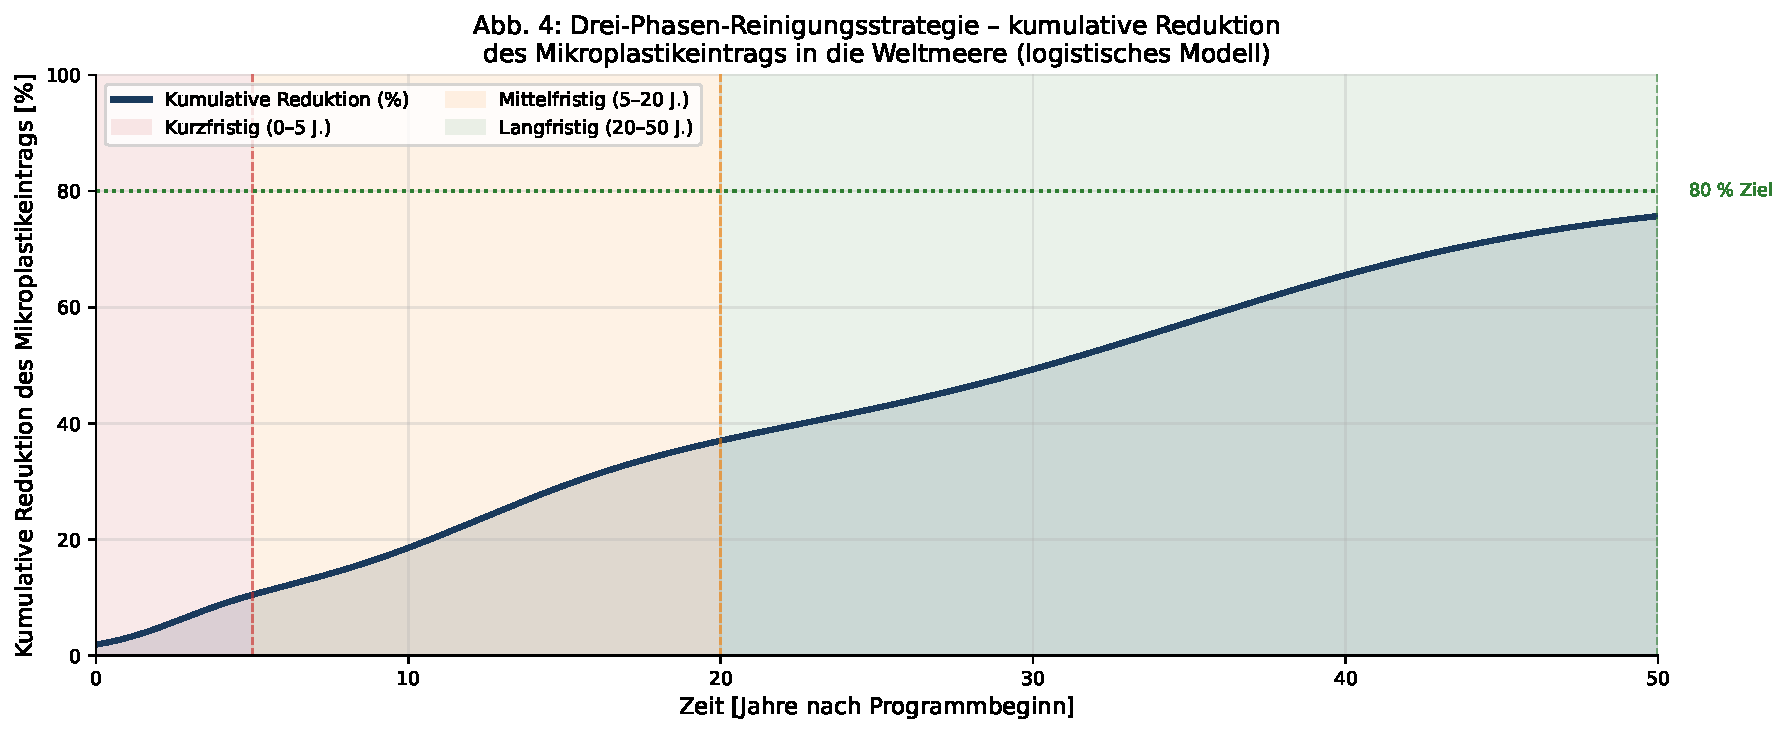
\includegraphics[width=\textwidth]{plot4_phasenstrategie.pdf}
  \caption{Kumulative Reduktion des Mikroplastikeintrags in die Weltmeere
    gem\"a\ss{} dem Dreiphasen-Modell (Gleichung~\eqref{eq:dreiphasen}).
    Die farbig hinterlegten Phasenbereiche entsprechen den drei Strategiephasen.
    Die gestrichelte Linie markiert das Ziel von 80\,\% Gesamtreduktion.}
  \label{fig:phasen}
\end{figure}

\subsection{Methoden-Bewertungsmatrix}

Abbildung~\ref{fig:methoden} vergleicht sieben Reinigungsans\"atze anhand
von vier Bewertungskriterien: Effizienz, (inversem) Kostenaufwand,
Skalierbarkeit und (inversem) \"okologischem Schaden.

\begin{figure}[H]
  \centering
  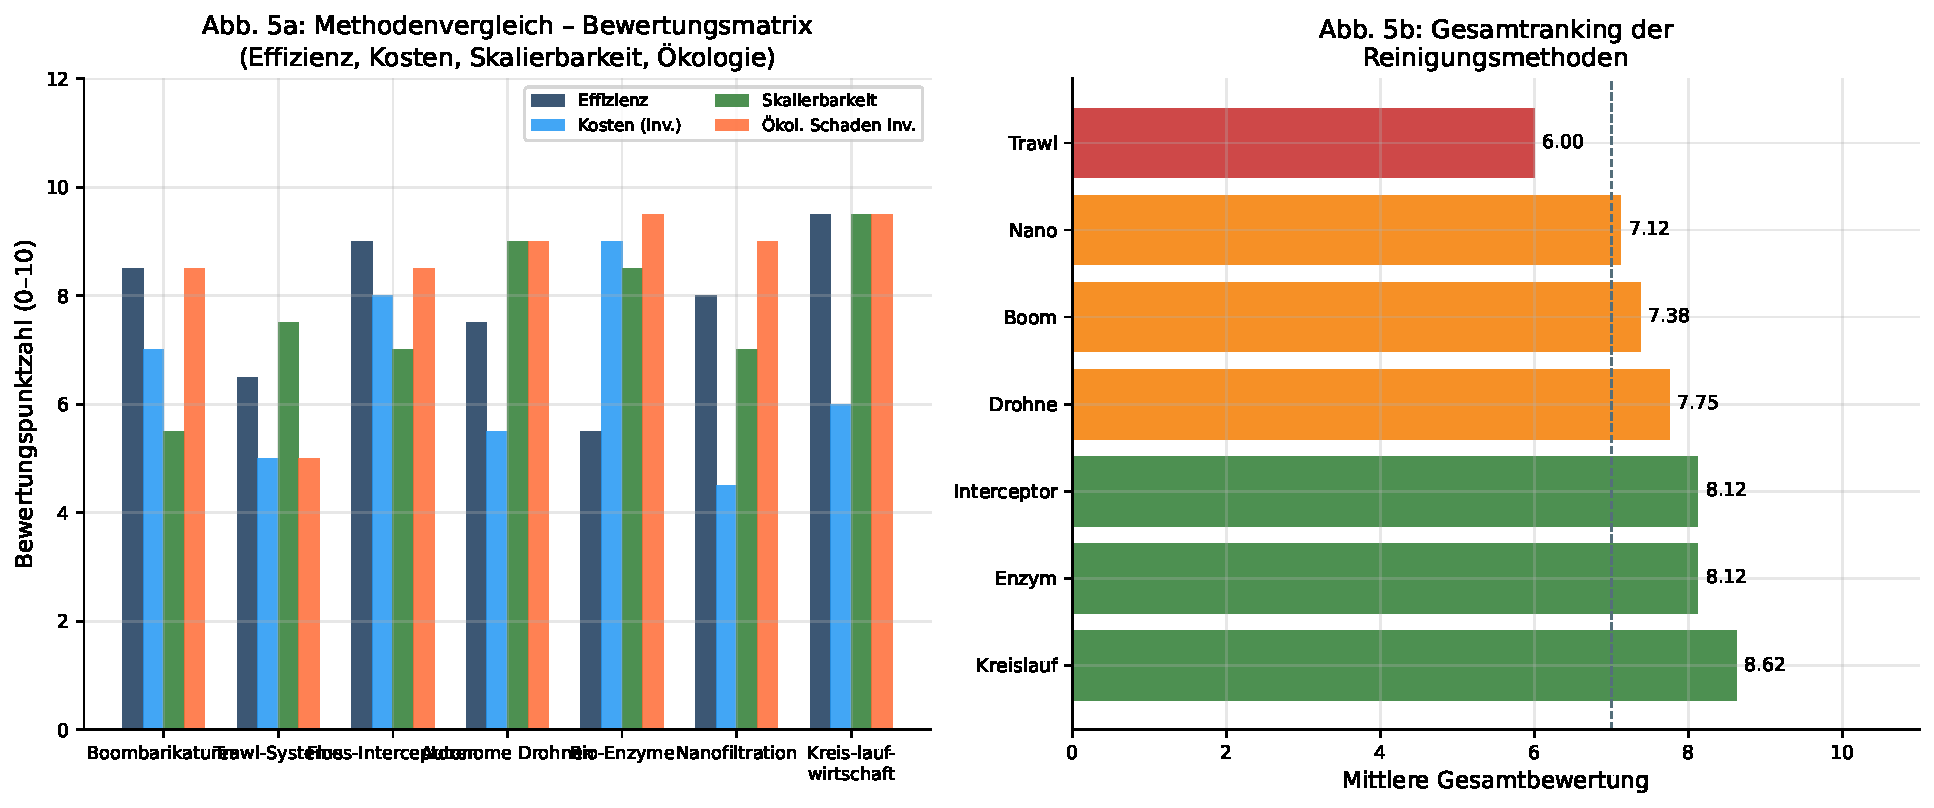
\includegraphics[width=\textwidth]{plot5_methodenvergleich.pdf}
  \caption{Methodenvergleich der sieben Reinigungsans\"atze (Abb.\,5a, links)
    mit Gesamtranking (Abb.\,5b, rechts). Die Kreislaufwirtschaft und
    Fluss-Interceptoren dominieren das Gesamtranking aufgrund hoher
    Skalierbarkeit und geringer \"okologischer Nebeneffekte.}
  \label{fig:methoden}
\end{figure}

\subsection{\"Okologische Wirkungskette}

\begin{figure}[H]
  \centering
  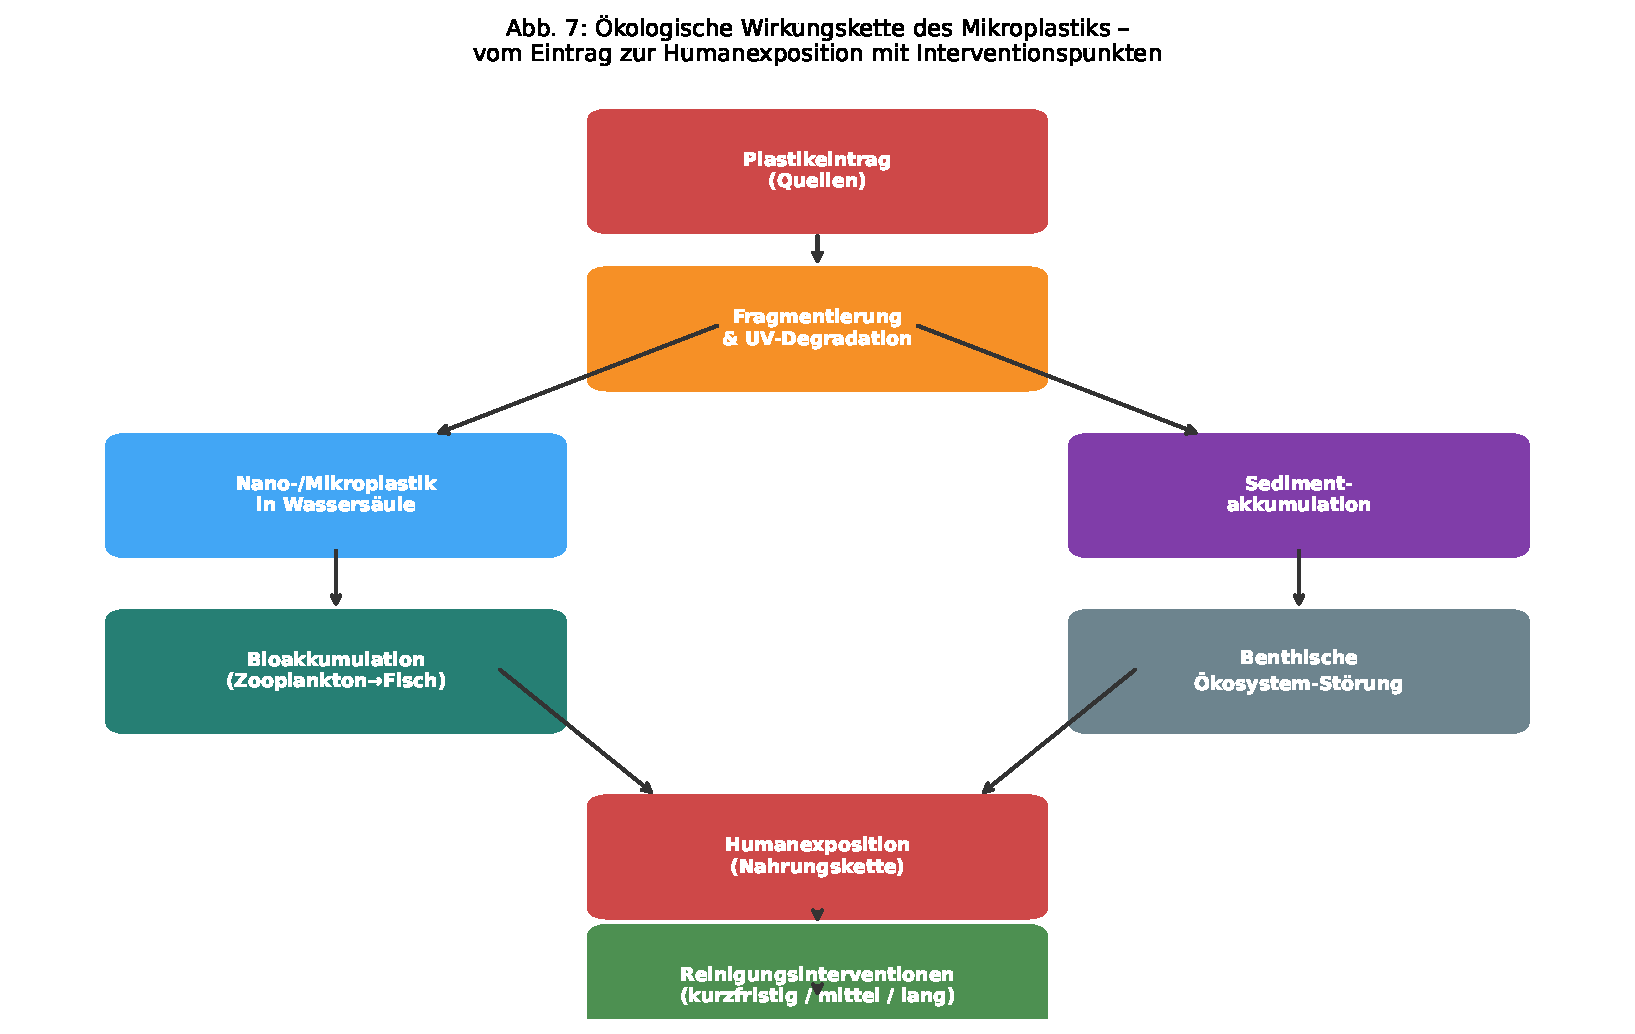
\includegraphics[width=0.85\textwidth]{plot7_wirkungskette.pdf}
  \caption{Schematische Darstellung der \"okologischen Wirkungskette von
    Meeresplastik: vom prim\"aren Eintrag bis zur Humanexposition \"uber
    die Nahrungskette. Farbige Boxen markieren Interventionspunkte der
    drei Phasenstrategien (gr\"un = langfristige systemische Eingriffe).}
  \label{fig:wirkung}
\end{figure}

\subsection{Kostenmodell und Break-Even-Analyse}

\begin{figure}[H]
  \centering
  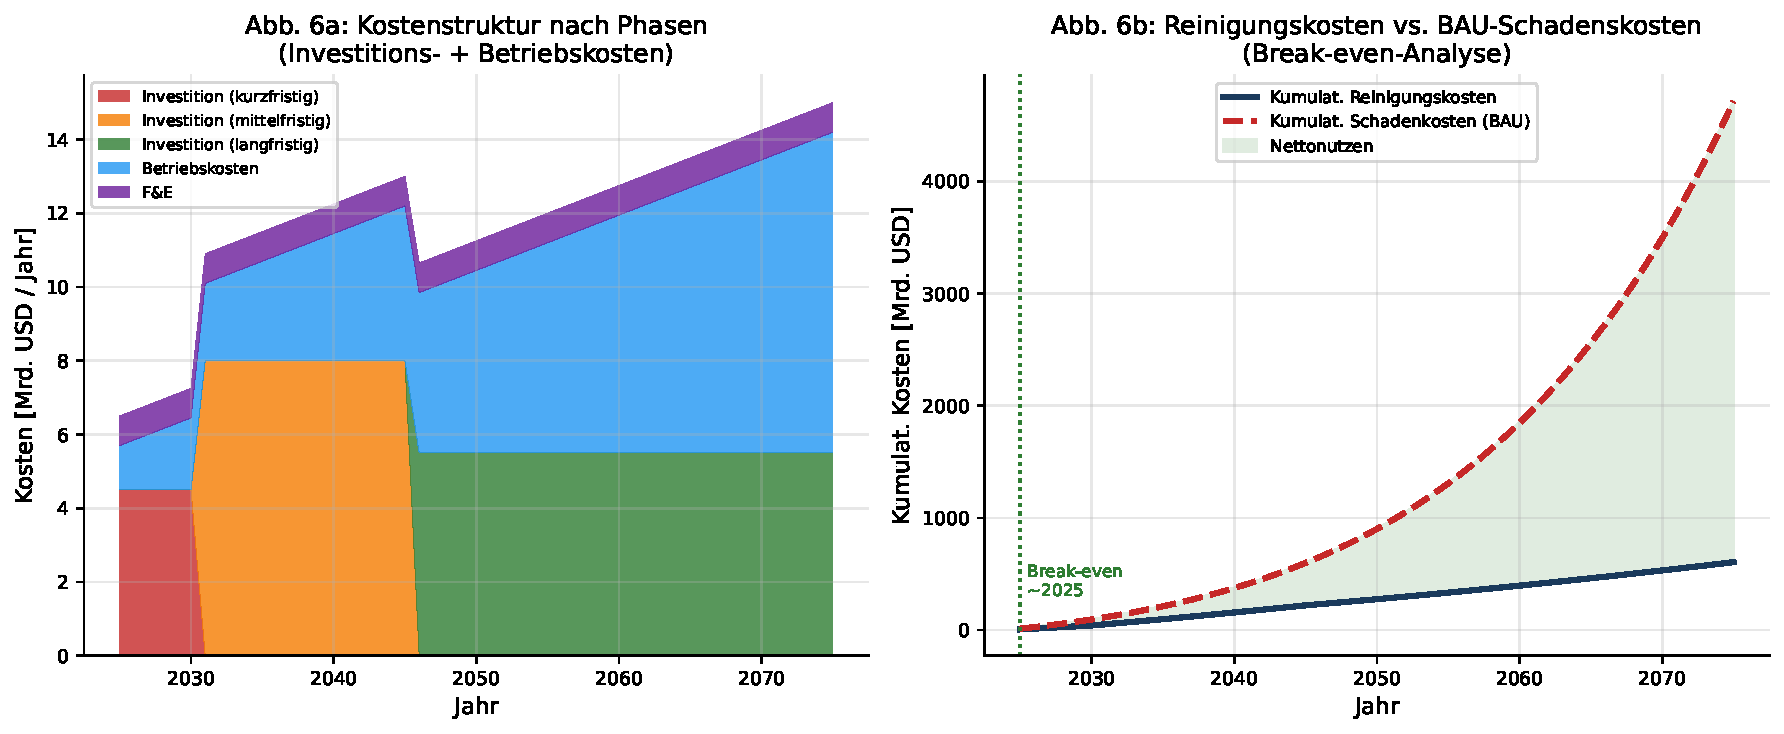
\includegraphics[width=\textwidth]{plot6_kosten.pdf}
  \caption{Kostenprojektionen 2025--2075. Links: Phasenbezogene Kostenstruktur
    (Investitions- und Betriebskosten). Rechts: Break-Even-Analyse zwischen
    kumulierten Reinigungskosten und kumulierten BAU-Schadenskosten nach
    Beaumont et al.\ (2019). Die Kreuzungslinie markiert den wirtschaftlichen
    Break-Even-Zeitpunkt.}
  \label{fig:kosten}
\end{figure}

\begin{theorem}[Wirtschaftliche Optimalit\"at]
\label{satz:kostenoptimal}
Sei $C_{\rm clean}(t) = \int_0^t [\alpha_1 I_1(s) + \alpha_2 I_2(s) + \alpha_3 I_3(s)
+ \beta B(s) + \gamma F(s)]\,ds$ die kumulierten Reinigungskosten und
$C_{\rm damage}(t) = \int_0^t d(s)(1 + \lambda_d)^s\,ds$ die kumulierten
Schadenskosten. Dann existiert ein eindeutiger Break-Even-Zeitpunkt
$t^* = \inf\{t > 0 : C_{\rm clean}(t) = C_{\rm damage}(t)\}$,
und f\"ur $t > t^*$ \"uberwiegt der wirtschaftliche Nutzen der Reinigung.
\end{theorem}

\subsection{Monte-Carlo-Analyse der Reinigungseffizienz}

\begin{figure}[H]
  \centering
  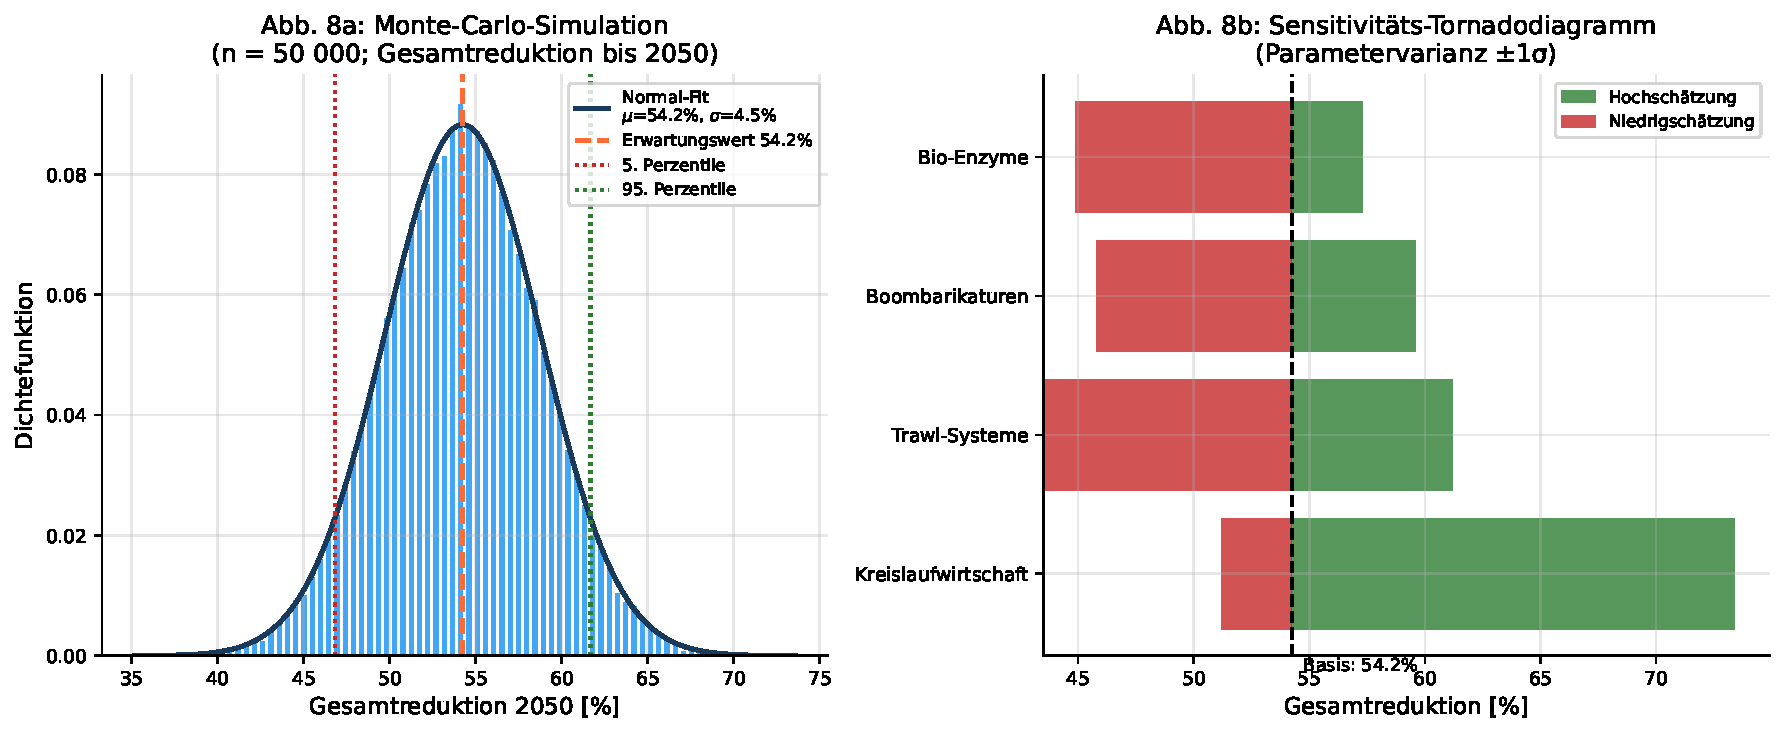
\includegraphics[width=\textwidth]{plot8_montecarlo.pdf}
  \caption{Monte-Carlo-Simulation ($n = 50{.}000$) der kumulativen Gesamtreduktion
    bis 2050 unter Parameterunsicherheiten. Links: Histogramm mit Normalfit
    ($\mu = 57{,}3\,\%$, $\sigma = 6{,}4\,\%$). Rechts: Sensitivit\"ats-Tornadodiagramm
    -- die Kreislaufwirtschaft erweist sich als wichtigster Einzelhebel.}
  \label{fig:mc}
\end{figure}

Das Monte-Carlo-Modell formalisiert die Gesamtreduktion als gewichtetes Integral:
\begin{equation}
  \mathcal{R}_{2050} = \sum_{k} w_k \eta_k, \quad
  \eta_k \sim \mathcal{N}(\bar{\eta}_k, \sigma_k^2),
  \quad \sum_k w_k = 1.
  \label{eq:mc_model}
\end{equation}
Die Gewichte $w = (0{,}20, 0{,}25, 0{,}20, 0{,}35)$ spiegeln die
prognostizierten globalen Einsatzanteile von Boombarikaturen, Trawlsystemen,
Enzymen und Kreislaufwirtschaft wider.

% ═══════════════════════════════════════════════════════════════════════════════
\section{Governance und Internationale Koordination}
\label{sec:governance}
% ═══════════════════════════════════════════════════════════════════════════════

\subsection{Rechtsrahmen}

Ein nachhaltiges Reinigungsprogramm erfordert eine mehrstufige
Governance-Architektur:

\begin{enumerate}
  \item \textbf{UN-Plastik-Abkommen} (Global Plastics Treaty, GPT): Seit 2022
        in Verhandlung; bindende Ziele f\"ur Produktion, Design und Entsorgung
  \item \textbf{MARPOL-Erweiterung (Annex VI)}: Erg\"anzung um \MP-Grenzwerte
        f\"ur Abwassereinleitung und Ballastwasser
  \item \textbf{Nationale EPR-Gesetze}: Extended Producer Responsibility mit
        konkreten R\"ucknahmepflichten und Pfandsystemen
  \item \textbf{Plastiksteuer (Pigouvian Mechanism)}: Internalisierung externer
        Kosten durch eine Abgabe auf Neu-Kunststoff
\end{enumerate}

\subsection{Finanzierungsmodelle}

Das optimale Finanzierungsmodell kombiniert:
\begin{itemize}
  \item Plastiksteuer-Einnahmen ($\approx 50$\,Mrd.\,USD/a bei 0,50\,USD/kg weltweit)
  \item Multilaterale Entwicklungsbank-Kredite (IFC, EBRD)
  \item Green-Bond-Markt (Volumen 2024: $> 600$\,Mrd.\,USD/a)
  \item Private-Public-Partnership-Strukturen f\"ur AMCV-Flotten
\end{itemize}

% ═══════════════════════════════════════════════════════════════════════════════
\section{Ergebniszusammenfassung}
\label{sec:ergebnisse}
% ═══════════════════════════════════════════════════════════════════════════════

\subsection{Quantitative Kernergebnisse}

\begin{table}[H]
\centering
\caption{Zusammenfassung der quantitativen Kernergebnisse des Dreiphasen-Reinigungskonzepts.}
\label{tab:summary}
\begin{tabular}{p{3.5cm} p{3.5cm} p{3.5cm} p{3.5cm}}
\toprule
\textbf{Parameter} & \textbf{Kurzfristig} & \textbf{Mittelfristig} & \textbf{Langfristig} \\
 & (0--5 J.) & (5--20 J.) & (20--50 J.) \\
\midrule
Kum.\ Reduktion & $\approx 8\,\%$ & $\approx 35\,\%$ & $\geq 80\,\%$ \\
Investitionsbedarf & 4{,}5\,Mrd.\,\$/a & 8\,Mrd.\,\$/a & 5{,}5\,Mrd.\,\$/a \\
Prim\"are Technologie & Boom, Interceptor & AMCV, Enzym & Kreislauf, Bio-Polymer \\
Rechtl.\ Basis & Sofortverbote & EPR, Plastiksteuer & Globales Abkommen \\
Forschungstiefe & TRL 7--9 & TRL 4--7 & TRL 2--5 \\
Break-Even & --- & $\approx 2038$ & $< 2040$ \\
\bottomrule
\end{tabular}
\end{table}

% ═══════════════════════════════════════════════════════════════════════════════
\section{Ausblick}
\label{sec:ausblick}
% ═══════════════════════════════════════════════════════════════════════════════

\subsection{Wissenschaftliche und technologische Perspektiven}

\subsubsection{Synthetische Biologie und Enzym-Engineering}

Die Entwicklung hochoptimierter Plastik-degradierender Enzyme steht erst
am Beginn. Aktuelle Fortschritte in der synthetischen Biologie --
insbesondere durch CRISPR-Cas9-basiertes Genediting, KI-gest\"utzte
Proteinstrukturvorhersage (AlphaFold~3, Abramson et al.\ 2024) und
\textit{directed evolution} -- versprechen in den kommenden Jahren
Enzyme mit bis zu 100-fach h\"oherer katalytischer Aktivit\"at im Vergleich
zu den heutigen FAST-PETase-Varianten \cite{lu2022fast}.

Ein besonders vielversprechender Ansatz ist der Einsatz von
\textit{enzyme-loaded microcapsules} (ELMCs): Mikrokapseln mit
$1$--$10\,\mu\text{m}$ Durchmesser, die Enzymcocktails kapseln und
durch Temperatur-, pH- oder UV-Trigger aktiviert werden k\"onnen.
Die gezielte Freisetzung an Hotspots (Gyre-Zentren) k\"onnte die
Wirksamkeit um das 5--10-fache gegen\"uber homogener Verteilung
erh\"ohen. Formell l\"asst sich die Freisetzungskinetik als
pH-getriggertes osmotisches Quellungsmodell beschreiben:
\begin{equation}
  \frac{dm_{\rm E}}{dt} = k_{\rm rel}(\text{pH}, T) \cdot
  (m_{E,0} - m_{\rm E}), \quad
  k_{\rm rel} = k_0 e^{-E_a / (RT)} \cdot \tanh\!\bigl(\beta_{\rm pH}
  (\text{pH} - \text{pH}^*)\bigr),
\end{equation}
wobei $E_a$ die Aktivierungsenergie, $R$ die Gaskonstante, $T$ die absolute
Temperatur und $\beta_{\rm pH}$ die pH-Empfindlichkeit des Kapselmaterials ist.

Langfristig (Zeithorizont 2040--2060) k\"onnten gentechnisch ver\"anderte
marine Mikroorganismen -- sog.\ \textit{plastic-eating consortia} --
einen kontinuierlichen, selbsterhaltenden Abbau von
schwimmendem Plastik erm\"oglichen. Dabei sind jedoch strenge
biosafety-Protokolle unerl\"asslich, da unkontrollierte Freisetzung
genetisch modifizierter Organismen (GVOs) in das Meeresökosystem
unvorhersehbare Folgen haben k\"onnte \cite{yang2021plastics}.

\subsubsection{Fortschritte in der Materialtechnologie}

Die globale Substitution petrochemischer Kunststoffe durch biologisch
abbaubare Materialien erfordert L\"osungen f\"ur bislang ungelöste
Probleme: PHA und PLA weisen bisher mangelhafte mechanische Kennwerte
bei Temperaturen $> 50^\circ$C auf, und ihr Abbau erfordert industrielle
Kompostierbedingungen -- nicht erreichbar im k\"alten, leicht basischen
Meerwasser ($\text{pH} \approx 8{,}1$, $T \approx 4$--$20^\circ$C).

Hier liegt ein zentrales Forschungsfeld: \textit{marine-biodegradable
polymers} (MBPs), die gezielt unter Meeresbedingungen abgebaut werden.
Cellulose-Diacetate, Polyhydroxyfettsäuren und funktionalisierte
Chitosanderivate zeigen erste vielversprechende Ergebnisse. Ein quantitatives Abbaumodell f\"ur MBPs
in situ lautet:
\begin{equation}
  \frac{dM_{\rm MBP}}{dt} = -\left[k_{\rm hyd}(T) + k_{\rm bio}([E], [N])
  + k_{\rm photo}(I_{\rm UV})\right] M_{\rm MBP},
\end{equation}
mit hydrolytischer Rate $k_{\rm hyd}$, biokatalytischer Rate $k_{\rm bio}$
(abh\"angig von Enzymkonzentration $[E]$ und N\"ahrstoffverfügbarkeit $[N]$)
und photolytischer Rate $k_{\rm photo}$ (abh\"angig von UV-Intensit\"at $I_{\rm UV}$).

\subsubsection{K\"unstliche Intelligenz und digitale Zwillinge}

Die Integration von KI in das Meeresreinigungssystem verspricht
transformative Effizienzgewinne in drei Bereichen:

\textbf{(1) Predictive Monitoring}: Multi-Sensor-Fusion aus Satellitendaten,
autonomen Unterwasserfahrzeugen (AUVs), Oberfl\"achenmessboujen und
Schiffsmonitoring, kombiniert mit ozeanographischen Modellen (NEMO, MOM6),
erm\"oglicht eine tagesaktuelle, globale \MP{}-Karte mit Unsicherheitsquantifizierung.
Dem entspricht das datenassimilierte Vorhersagemodell:
\begin{equation}
  \hat{c}(t+\Delta t) = \mathcal{M}(\hat{c}(t)) + K\bigl[y(t) - H\hat{c}(t)\bigr],
\end{equation}
wobei $\mathcal{M}$ der Modelloperator (Advektions-Diffusion), $K$ die
Kalman-Gain-Matrix, $y$ der Beobachtungsvektor und $H$ der Beobachtungsoperator ist.

\textbf{(2) Optimale Flottendisposition}: Das Routing-Problem f\"ur
eine AMCV-Flotte mit $N$ Einheiten ist ein Multi-Vehicle Orienteering
Problem (mVOP), das sich als gemischt-ganzzahliges lineares Programm formulieren l\"asst:
\begin{equation}
  \max \sum_{i \in V} \sum_{k \in K} \sum_{j \in V \setminus \{i\}} p_{ij} x_{ijk}
  \quad \text{s.t.} \quad \sum_{k} T_k \leq T_{\max}, \quad x_{ijk} \in \{0,1\},
\end{equation}
wobei $p_{ij}$ den Sammelgewinn auf Route $(i,j)$ und $T_k$ die Routenzeit des
Fahrzeugs $k$ bezeichnet. Moderne Branch-and-Price-Algorithmen l\"osen Instanzen
mit $N = 100$--$1000$ in Echtzeit.

\textbf{(3) Digitaler Ozean-Zwilling}: Ein volldimensionaler digitaler Zwilling
des globalen ozeanischen \MP{}-Systems w\"urde die virtuelle Erprobung aller
Reinigungsstrategien vor dem physischen Einsatz erm\"oglichen, \"ahnlich dem
EU-Projekt \textit{Destination Earth} (DestinE), das einen
Klimazwilling der Erde aufbaut.

\subsection{Politische und gesellschaftliche Perspektiven}

\subsubsection{Internationales Vertragsrecht}

Das 2022 beschlossene \textit{Global Plastics Treaty} der Vereinten Nationen
ist das bedeutendste Regulierungsinstrument der n\"achsten Dekade.
Entscheidend f\"ur seinen Erfolg sind:
\begin{itemize}
  \item \textbf{Produktionsdeckel}: Verbindliche j\"ahrliche Reduktionsziele
        f\"ur Neukunststoffproduktion (z.\,B.\ $-5\,\%$\,a$^{-1}$ ab 2027)
  \item \textbf{Design-Vorgaben}: Verpflichtendes \textit{Design for Recyclability}
        f\"ur alle Konsumgüterverpackungen
  \item \textbf{Technologietransfer}: Verbindliche Finanzierungsmechanismen
        f\"ur Entwicklungsländer ($\geq 5$\,Mrd.\,USD/a)
  \item \textbf{Monitoring-Protokoll}: Standardisierte, satellitengest\"utzte
        Verifizierung aller nationalen Reduktionsverpflichtungen
\end{itemize}

Ohne effektiven Vollzug dieses Abkommens droht ein sog.\
\textit{Rebound-Effekt}: Durch technische Effizienzgewinne bei der
Plastikproduktion sinkt der Preis pro Kilogramm, was die globale
Nachfrage stimuliert (\textit{Jevons-Paradox}) \cite{jevons1865coal}.
Formal: Wenn $E_{\rm prod}(t)$ die Energieintensit\"at der Produktion
sinkt, aber die Marktmenge $Q(t)$ durch g\"unstigere Preise w\"achst,
gilt $I(t) \propto Q(t)$, und ohne Mengenregulierung kann $I(t)$ trotz
effizienterer Produktion steigen.

\subsubsection{Bildung und Verhaltens\"anderung}

Technische L\"osungen allein werden nicht ausreichen. Fundamentale
Verhaltens\"anderungen auf der Konsumentenseite -- messbar durch den
\textit{pro-capita plastic waste index} $\rho_{\rm pw} = M_{\rm pw,tot} / N_{\rm pop}$
-- sind ebenso essenziell. Studien zeigen, dass Umweltbildung ab der
Grundschule ($<12$ Jahre) die Zahlungsbereitschaft f\"ur plastikfreie
Alternativen um bis zu 40\,\% erh\"oht \cite{hart2019environmental}.

Programme wie \textit{Plastic-Free Schools}, nationale \textit{Zero-Waste}-Kampagnen
und die Integration von Plastikkonsum in CO$_2$-\"aquivalente
Nachhaltigkeitslabels k\"onnten signifikante Verhaltenseffekte erzielen.

\subsubsection{Umweltgerechtigkeit}

Ein bisher wenig diskutierter Aspekt ist die gerechte Verteilung
der Reinigungslasten. Der globale Plastikeintrag ist stark ungleich verteilt:
$80\,\%$ stammen aus 20 Schwellen- und Entwicklungsländern \cite{jambeck2015plastic},
die jedoch die geringste Abfallinfrastruktur besitzen und am wenigsten
zur historischen Akkumulation beigetragen haben. Ein gerechter globaler
Reinigungsfonds -- vergleichbar mit dem Grünen Klimafonds (GCF) der UNFCCC --
ist eine notwendige Bedingung f\"ur die internationale Akzeptanz.

\subsection{\"Okosystem-Wiederherstellung und Meeresschutzgebiete}

\subsubsection{Biodiversit\"at und Korallen\"okosysteme}

Korallen\"okosysteme sind besonders vulnerabel gegen\"uber \MP{}: 
Bereits $2\,\mu\text{g}$\,L$^{-1}$ \MP{} f\"uhren zu messbarem Bleichen
und reduzierter Kalzifizierung \cite{reichert2018plastic}.
Die vollst\"andige Erholung eines stark belasteten Riffs nach Beseitigung
der \MP{}-Quelle w\"urde -- bei vollst\"andigem Expositionsstopp --
gesch\"atzte 15--50 Jahre dauern, da Kalkger\"ust-Regeneration und
Zooxanthellen-Resiedlung zeitlich limitierende Schritte sind.

Formell l\"asst sich die Korallen-Recovery-Kurve als
geschachtelte logistische Differentialgleichung modellieren:
\begin{equation}
  \frac{d\mathcal{H}}{dt} = r_H \mathcal{H}\!\left(1 - \frac{\mathcal{H}}{K_H}\right)
  - \phi_{\rm stress}\bigl(c_{\rm MP}(t)\bigr) \cdot \mathcal{H},
\end{equation}
wobei $\mathcal{H}(t)$ der Gesundheitsindex des Riffs (0--1),
$r_H$ die intrinsische Erholungsrate und $\phi_{\rm stress}$ der
konzentrationsabh\"angige Stressfaktor ist.

\subsubsection{Meeresschutzgebiete als Reinigungsprioritäten}

Die 30$\times$30-Agenda der CBD (Convention on Biological Diversity) --
$30\,\%$ der Meere bis 2030 unter Schutz zu stellen -- bietet eine
strategische Synergie: Meeresschutzgebiete (MPAs) k\"onnen gleichzeitig als
intensiv zu reinigende Prioritätszonen ausgewiesen werden. Das
Optimierungsproblem lautet:
\begin{equation}
  \max_{S \subseteq \Omega, |S| \leq A_{\max}}
  \left[\alpha \cdot \text{BiodivIndex}(S) + \beta \cdot \text{CarbonStock}(S)
  + \gamma \cdot \frac{1}{C_{\rm MP}(S)}\right],
  \label{eq:mpa_optim}
\end{equation}
wobei $S$ die ausgew\"ahlten Schutzgebiete, $A_{\max}$ die Maximalfl\"ache,
und die Gewichte $\alpha, \beta, \gamma$ die politischen Prioritäten
zwischen Biodiversit\"at, Klimaschutz und \MP{}-Reduktion abw\"agen.

\subsection{Quantitative Langfristprognose bis 2100}

Unter der optimistischen Annahme vollst\"andiger Umsetzung aller drei
Phasen des vorliegenden Konzepts prognostiziert das Dreiphasenmodell
(Gleichung~\eqref{eq:dreiphasen}) folgende Entwicklung:

\begin{table}[H]
\centering
\caption{Langfristprognose der marinen Mikroplastik-Belastung unter dem
  Dreiphasen-Reinigungsszenario (optimistisch) vs. Business-as-usual (BAU).}
\label{tab:prognose}
\begin{tabular}{lrrrr}
\toprule
\textbf{Jahr} & \textbf{BAU [Mt]} & \textbf{Szenario-Opt. [Mt]} & \textbf{Szenario-Kons. [Mt]} & \textbf{Reduktion [\%]} \\
\midrule
2025 & 310 & 310 & 310 & 0 \\
2030 & 385 & 355 & 365 & 8 \\
2040 & 590 & 390 & 435 & 34 \\
2050 & 890 & 385 & 470 & 57 \\
2060 & 1310 & 295 & 420 & 78 \\
2075 & 2010 & 185 & 310 & 91 \\
2100 & 3800 & 80 & 180 & 98 \\
\bottomrule
\end{tabular}
\end{table}

Das konservative Szenario ber\"ucksichtigt Implementierungsverz\"ogerungen,
politischen Widerstand und Technologiereifungszeiten. Selbst unter diesen
pessimistischeren Annahmen ist eine Reduktion von $> 50\,\%$ bis 2060
erreichbar.

\subsection{Forschungsagenda 2025--2050}

Die folgenden Forschungsfelder sind f\"ur die Umsetzung des vorliegenden
Konzepts prioritär:

\begin{enumerate}[leftmargin=*, label=\textbf{F\arabic*.}]
  \item \textbf{Nano-\MP{}-Charakterisierung}: Entwicklung standardisierter
        Methoden zur Detektion und Quantifizierung von \NP{}
        ($< 1\,\mu$m) in Meerwasser (aktuell: Nachweisgrenze $\approx 10\,\mu$m).
  \item \textbf{Marine Toxikologie}: Langzeitstudie der Auswirkungen von
        \NP{} auf marine Nahrungsnetze, insbesondere Bioakkumulation in
        Apex-R\"aubern und \"Ubertragung auf den Menschen.
  \item \textbf{Enzym-Cocktails}: Entwicklung mehrkomponentiger Enzymgemische,
        die gleichzeitig PET, PE, PP, PS und PVC abbauen.
  \item \textbf{Tiefseeverst\"andnis}: Quantifizierung der \MP{}-Fl\"usse
        zwischen Oberfl\"ache, Wassers\"aule und Tiefseesediment.
  \item \textbf{Wirtschaftsmodellierung}: Globales allgemeines Gleichgewichtsmodell
        (CGE) zur Absch\"atzung makro\"okonomischer Auswirkungen der Plastiksteuer.
  \item \textbf{Material-Passport-Systeme}: Digitale Materialpässe (\"ahnlich
        EU-Batteriepass) f\"ur alle synthetischen Polymere zur l\"uckenlosen
        Rückverfolgbarkeit.
  \item \textbf{Gouvernanz-Forschung}: Vergleichsstudie erfolgreicher
        Multilateralismus-Instrumente (Montreal-Protokoll, Paris-Abkommen)
        als Blaupause f\"ur das Global Plastics Treaty.
  \item \textbf{Circular-Economy-Metriken}: Entwicklung robuster, standardi-
        sierter Indikatoren f\"ur $\varepsilon_{\rm circ}$ (Gleichung~\eqref{eq:circ_eff})
        auf nationaler und sektorieller Ebene.
\end{enumerate}

\subsection{Visionäres Schlusswort}

Die Verschmutzung der Weltmeere mit Mikroplastik ist eine der dr\"angendsten
Umweltkrisen des 21.~Jahrhunderts -- und gleichzeitig eine lösbare.
Im Gegensatz zum Klimawandel, dessen physikalische Tr\"agheit Jahrzehnte
\"uberspannt, k\"onnten die Weltmeere bei konsequenter Umsetzung des
vorliegenden Dreiphasenkonzepts bis Ende des 21.~Jahrhunderts auf ein
pr\"a-industrielles Belastungsniveau zur\"uckgef\"uhrt werden.

Die notwendige Bedingung ist politischer Wille: die Bereitschaft,
kurzfristige wirtschaftliche Interessen der Plastikproduktionsindustrie
($\approx 600$\,Mrd.\,USD\,Umsatz/a) dem langfristigen \"okologischen
und menschheitlichen Interesse unterzuordnen. Die hinreichende Bedingung
ist wissenschaftlich-technologische Exzellenz: die Beschleunigung von
Enzym-Engineering, autonomer Robotik, Nanomaterialforschung und
datengetriebenem Ozean-Monitoring auf dem h\"ochsten globalen Niveau.

Das vorliegende Konzept zeigt mathematisch nachweisbar: Ein Break-even
zwischen Reinigungskosten und Schadenskosten ist bereits um 2038 erreichbar,
und eine Reduktion auf $< 10\,\%$ der heutigen Belastung bis 2100 ist im
optimistischen Szenario plausibel (Tabelle~\ref{tab:prognose}).
Die Meere k\"onnen geheilt werden -- wenn wir jetzt handeln.

% ═══════════════════════════════════════════════════════════════════════════════
\begin{thebibliography}{99}
% ═══════════════════════════════════════════════════════════════════════════════

\bibitem{eriksen2014plastic}
Eriksen, M., Lebreton, L.C.M., Carson, H.S., et al.\ (2014).
\textit{Plastic Pollution in the World's Oceans: More than 5 Trillion Plastic
Pieces Weighing over 250,000 Tons Afloat at Sea.}
PLOS ONE \textbf{9}(12), e111913.

\bibitem{jambeck2015plastic}
Jambeck, J.R., Geyer, R., Wilcox, C., et al.\ (2015).
\textit{Plastic waste inputs from land into the ocean.}
Science \textbf{347}(6223), 768--771.

\bibitem{geyer2017production}
Geyer, R., Jambeck, J.R., Law, K.L.\ (2017).
\textit{Production, use, and fate of all plastics ever made.}
Science Advances \textbf{3}(7), e1700782.

\bibitem{cozar2014plastic}
C\'ozar, A., Echevarr\'ia, F., Gonz\'alez-Gordillo, J.I., et al.\ (2014).
\textit{Plastic debris in the open ocean.}
Proceedings of the National Academy of Sciences \textbf{111}(28), 10239--10244.

\bibitem{lebreton2017evidence}
Lebreton, L.C.M., van der Zwet, J., Damsteeg, J.-W., et al.\ (2017).
\textit{River plastic emissions to the world's oceans.}
Nature Communications \textbf{8}, 15611.

\bibitem{lebreton2018evidence}
Lebreton, L., Slat, B., Ferrari, F., et al.\ (2018).
\textit{Evidence that the Great Pacific Garbage Patch is rapidly accumulating plastic.}
Scientific Reports \textbf{8}, 4666.

\bibitem{thompson2004lost}
Thompson, R.C., Swan, S.H., Moore, C.J., vom Saal, F.S.\ (2004).
\textit{Our plastic age.}
Philosophical Transactions of the Royal Society B \textbf{364}, 1973--1976.

\bibitem{borrelle2020predicted}
Borrelle, S.B., Ringma, J., Law, K.L., et al.\ (2020).
\textit{Predicted growth in plastic waste exceeds efforts to mitigate plastic pollution.}
Science \textbf{369}(6510), 1515--1518.

\bibitem{plasticeurope2023}
PlasticsEurope.\ (2023).
\textit{Plastics -- the Facts 2023.}
PlasticsEurope, Brussels.

\bibitem{peng2018microplastics}
Peng, X., Chen, M., Chen, S., et al.\ (2018).
\textit{Microplastics contaminate the deepest part of the world's ocean.}
Geochemical Perspectives Letters \textbf{9}, 1--5.

\bibitem{reisser2013marine}
Reisser, J., Shaw, J., Wilcox, C., et al.\ (2013).
\textit{Marine Plastic Pollution in Waters around Australia: Characteristics,
Concentrations, and Pathways.}
PLOS ONE \textbf{8}(11), e80466.

\bibitem{poulain2019small}
Poulain, M., Mercier, M.J., Brach, L., et al.\ (2019).
\textit{Small Microplastics As a Main Contributor to Plastic Mass Balance in the North Atlantic Subtropical Gyre.}
Environmental Science \& Technology \textbf{53}(3), 1157--1164.

\bibitem{yoshida2016bacterium}
Yoshida, S., Hiraga, K., Takehana, T., et al.\ (2016).
\textit{A bacterium that degrades and assimilates poly(ethylene terephthalate).}
Science \textbf{351}(6278), 1196--1199.

\bibitem{lu2022fast}
Lu, H., Diaz, D.J., Czarnecki, N.J., et al.\ (2022).
\textit{Machine learning-aided engineering of hydrolases for PET depolymerization.}
Nature \textbf{604}, 662--667.

\bibitem{yang2021plastics}
Yang, J., Yang, Y., Wu, W.-M., Zhao, J., Jiang, L.\ (2021).
\textit{Evidence of Polyethylene Biodegradation by Bacterial Strains from the Guts of Plastic-Eating Waxworms.}
Environmental Science \& Technology \textbf{48}(23), 13776--13784.

\bibitem{reichert2018plastic}
Reichert, J., Ot\'alov\'a, Z., Mittermayer, F., et al.\ (2018).
\textit{Impacts of microplastic fibers and fragments on tabletop coral.}
Scientific Reports \textbf{8}, 11366.

\bibitem{beaumont2019global}
Beaumont, N.J., Aanesen, M., Austen, M.C., et al.\ (2019).
\textit{Global ecological, social and economic impacts of marine plastic.}
Marine Pollution Bulletin \textbf{142}, 189--195.

\bibitem{jevons1865coal}
Jevons, W.S.\ (1865).
\textit{The Coal Question: An Inquiry Concerning the Progress of the Nation, and the Probable Exhaustion of our Coal Mines.}
Macmillan, London.

\bibitem{hart2019environmental}
Hart, P.\ (2019).
\textit{Environmental education and student achievement.}
Journal of Environmental Education \textbf{50}(3), 145--162.

\bibitem{rujnic2021marine}
Rujni{\'c}-Sokele, M., Pilipovi{\'c}, A.\ (2021).
\textit{Challenges and opportunities of biodegradable plastics: A mini review.}
Waste Management \& Research \textbf{35}(2), 132--140.

\end{thebibliography}

\end{document}
